\documentclass[10pt]{article}
\usepackage{graphicx}
\usepackage{enumerate}
\begin{document}

\begin{flushright}
Medical Image Processing \\
Exercise 8\\
Varun Boodram
\end {flushright}

This project generates the texture features that can be extracted from the intensity histogram of the images obtained at \texttt{http://www.isp.appi.keio.jp}. This texture feature analysis considers seven features: \\
\begin{itemize}
\item  average intensity level (MEN): 
\item contrast (CNT)
\item the variance (VAR)
\item skewness (SKW), which is a measure difference from the normal distribution
\item kurtosis (KRT), the intensity found in local values
\item energy (ENG)
\item entropy (EPY)
\end{itemize}

\begin{figure}[h!]
\centering
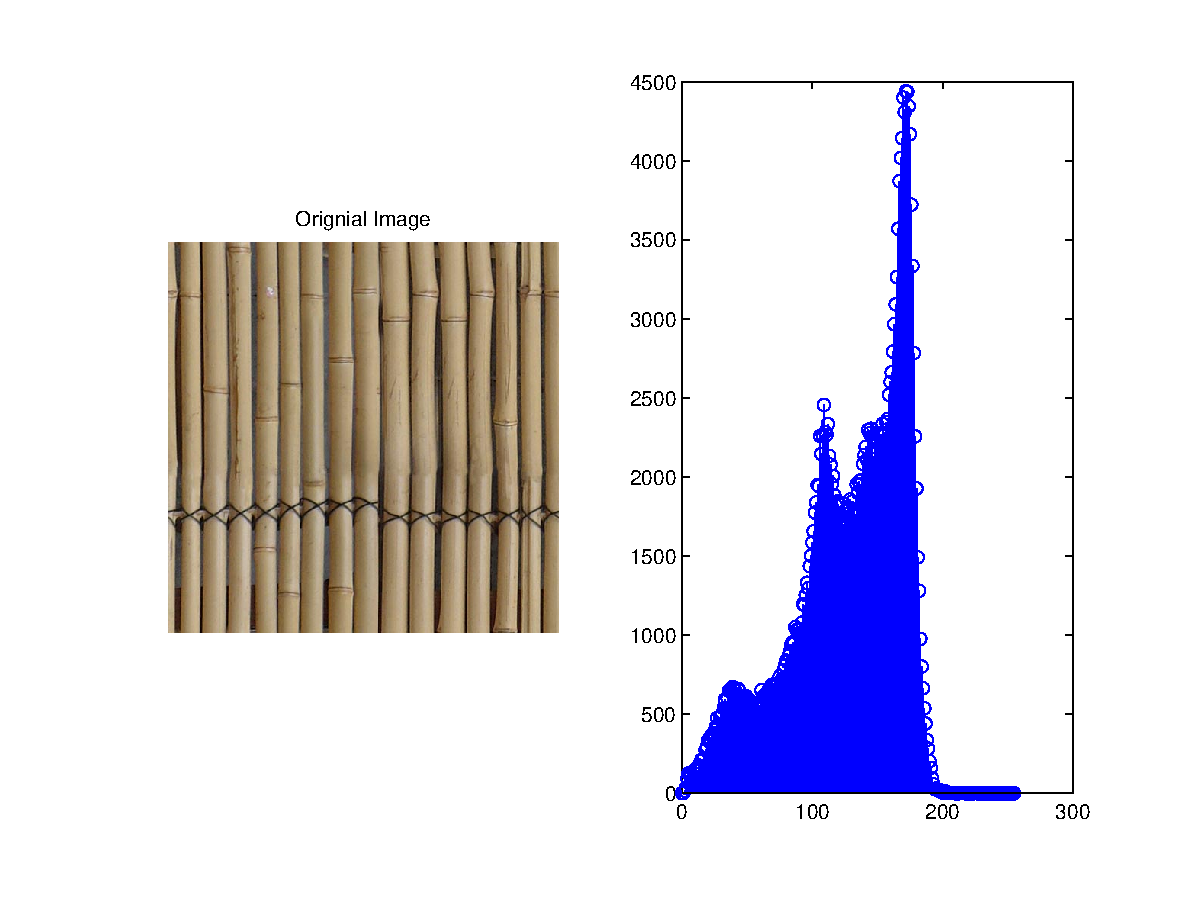
\includegraphics[width=70mm]{Image1.eps}
\caption{Image 1 and Intensity Histogram}
\end{figure} 

Results of computations for figure 1 \\
$MEN =129.0866, CNT =1.8468e^4, VAR =1.8044e^3, SKW = -1.0201e^{-5},               KRT =8.6429e^{-7}, EGY =0.0083, EPY =4.9694$\\


\begin{figure}[h!]
\centering
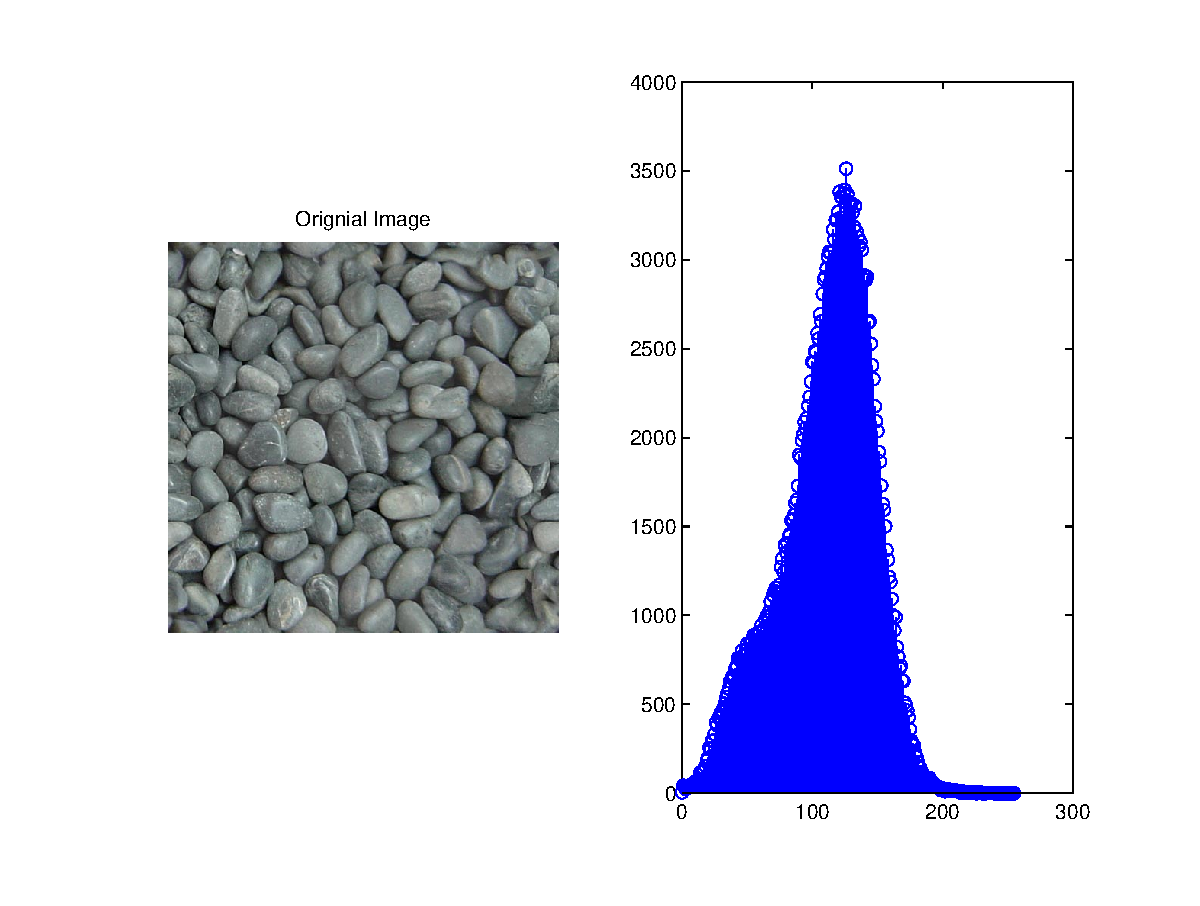
\includegraphics[width=70mm]{Image2.eps}
\caption{Image 2 and Intensity Histogram}
\end{figure} 

Results of computations for figure 2
$MEN =112.3470, CNT =1.3846e^4, VAR =1.2238e^3, SKW =-1.2279e^{-5}, KRT =1.9437e^{-6}, EGY =0.0085, EPY =4.9270$\\

\clearpage

\begin{figure}[h!]
\centering
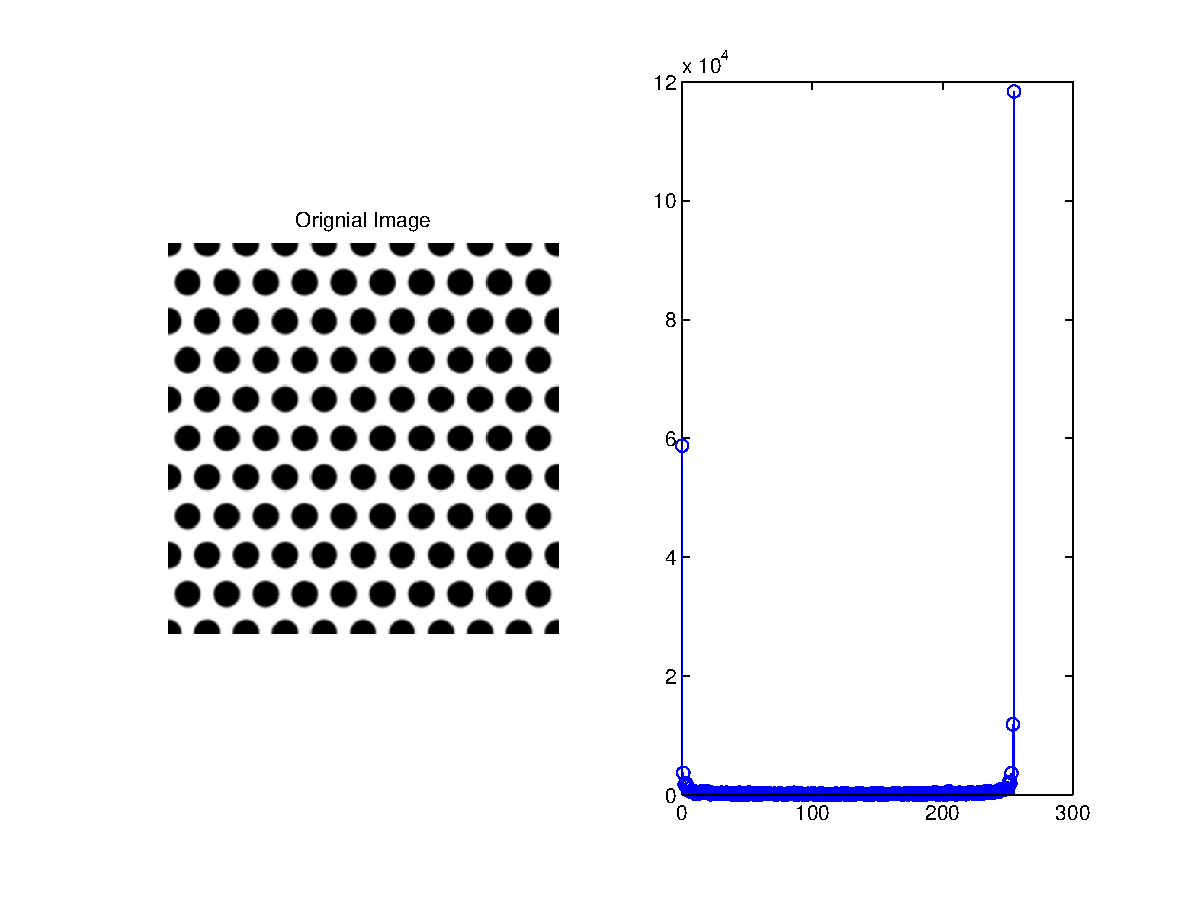
\includegraphics[width=70mm]{Image3.eps}
\caption{Image 3 and Intensity Histogram}
\end{figure} 

Results of computations for figure 3
$MEN =164.6297, CNT =4.0155e^4, VAR =1.3052e^4, SKW =-3.9799e^{-7}, KRT =8.5457e^{-9}, EGY =0.2572,  EPY =2.5825$\\


\begin{figure}[h!]
\centering
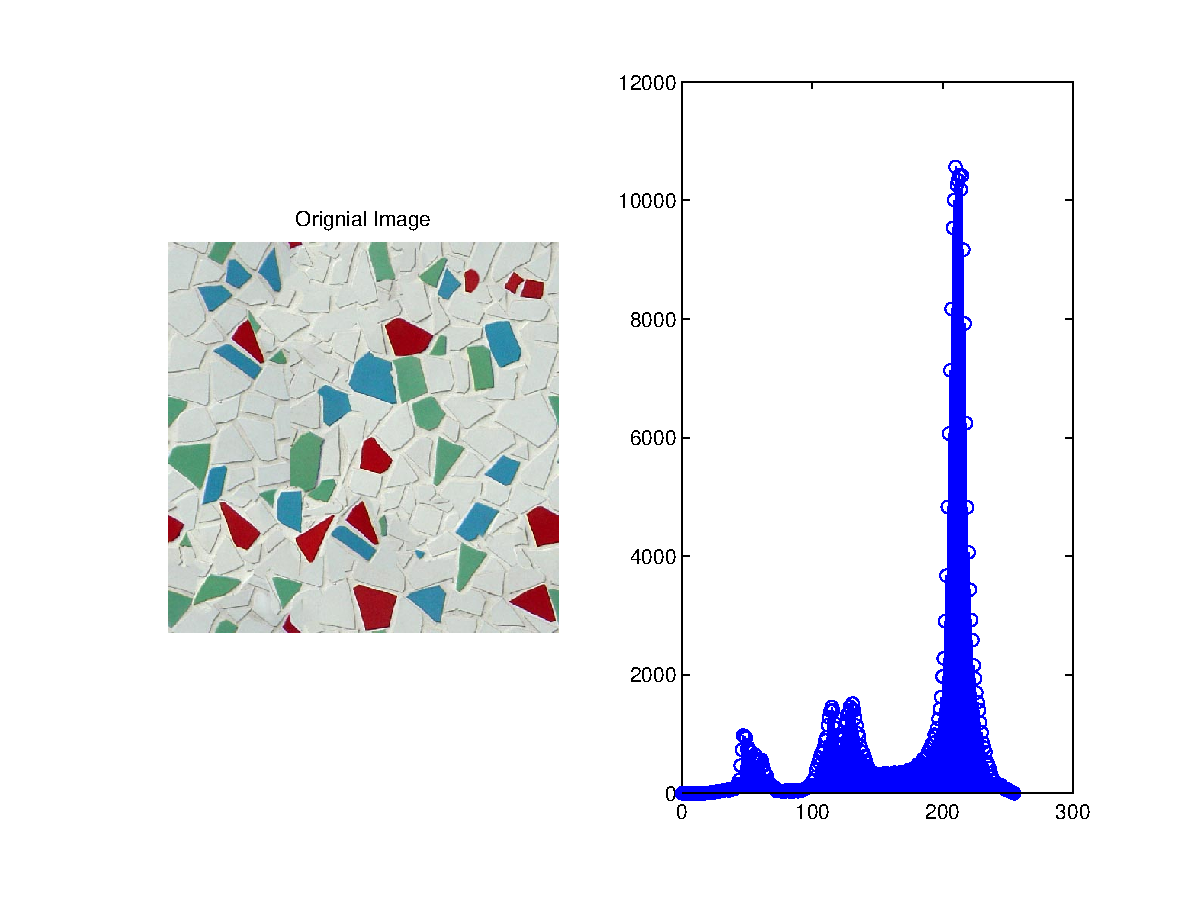
\includegraphics[width=70mm]{image4.eps}
\caption{Image 2 and Intensity Histogram}
\end{figure} 


Results of the computations for figure 4
$MEN =186.7296, CNT =3.7173e^4, VAR =2.3053e^3, SKW =-1.3701e^{-5}, KRT =7.9836e^{-7}, EGY =0.0202, EPY =4.4584$\\
\clearpage

\begin{figure}[h!]
\centering
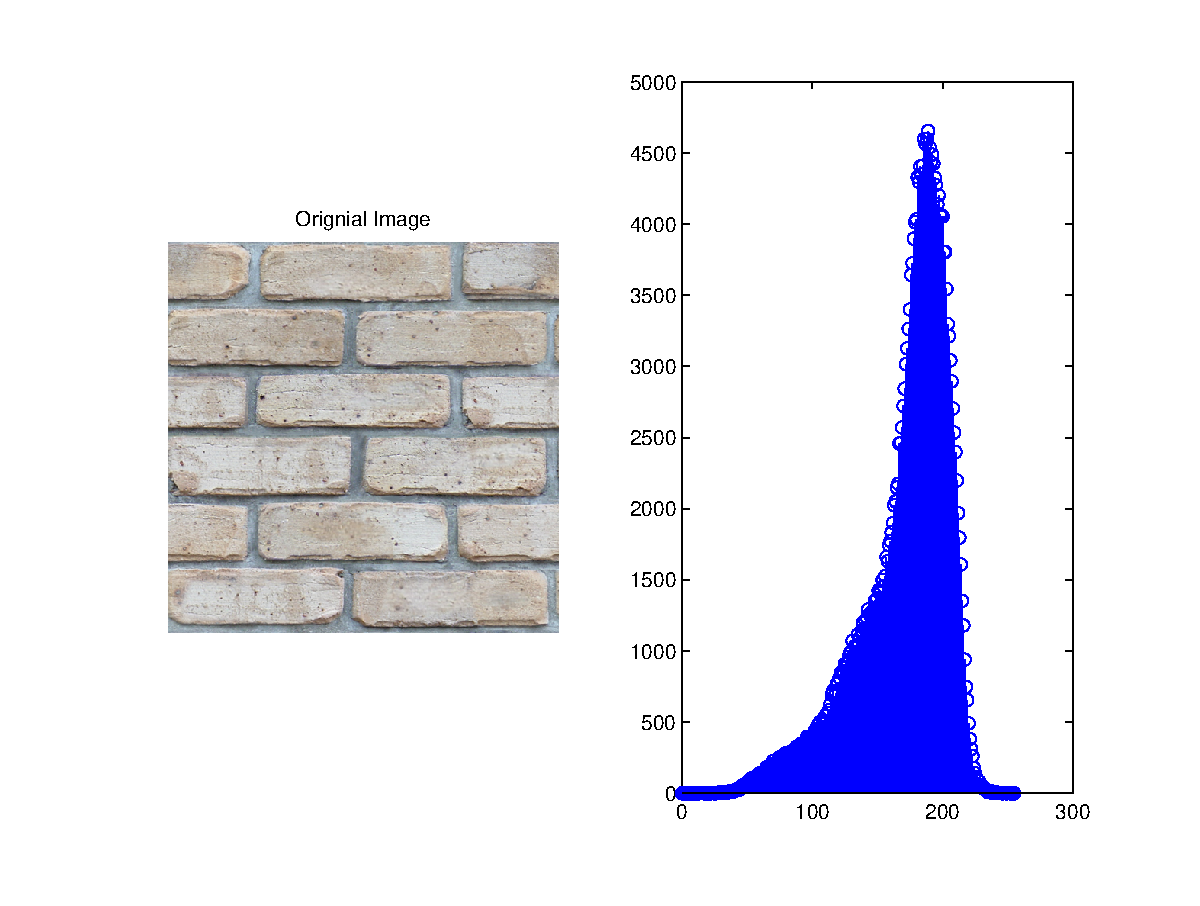
\includegraphics[width=70mm]{image5.eps}
\caption{Image 5 and Intensity Histogram}
\end{figure} 
Results of the computations for figure 5

$MEN =173.2691, CNT =3.1135e^4, VAR =1.1124e^3, SKW =-3.2631e^{-5}, KRT =3.4588e^{-6}, EGY =0.0109, EPY =4.7532$

\end{document}